% Canonical manuscript source. Edit this file directly.
% Writing rules: no em dashes, no semicolons, no self-assessment adjectives.
\documentclass[11pt,a4paper]{article}
\usepackage[T1]{fontenc}
\usepackage[utf8]{inputenc}
\usepackage{newtxtext,newtxmath}
\usepackage[margin=25mm]{geometry}
\usepackage{microtype}
\usepackage{amsmath}
\usepackage{graphicx}
\usepackage{booktabs}
\usepackage[font=small,labelfont=bf]{caption}
\usepackage[numbers,sort&compress]{natbib}
\PassOptionsToPackage{obeyspaces}{url}
\usepackage{xurl}
\usepackage[hidelinks]{hyperref}
\hypersetup{
  pdftitle={TorchFDTD: GPU finite-difference time-domain simulation with discrete adjoints and tiered-memory execution for photonic design},
  pdfauthor={Hyoseok Park},
  pdfsubject={Computational photonics software}
}
\newcommand{\code}[1]{{\small\nolinkurl{#1}}}
\newcommand{\micron}{\ensuremath{\mu\mathrm{m}}}
\setlength{\parskip}{3pt}
\setlength{\emergencystretch}{1.5em}
\setlength{\bibsep}{5pt}
\raggedbottom
\clubpenalty=10000
\widowpenalty=10000
\displaywidowpenalty=10000
\renewcommand{\topfraction}{0.85}
\renewcommand{\bottomfraction}{0.8}
\renewcommand{\textfraction}{0.1}
\renewcommand{\floatpagefraction}{0.75}
% Generated from docs/validation/flux.json.
\newcommand{\SlabTError}{0.00153444}
\newcommand{\SlabRError}{0.00153535}
\newcommand{\SlabEnergyError}{4.43991\times10^{-6}}


\title{\Large\bfseries TorchFDTD: GPU finite-difference time-domain simulation with discrete adjoints and tiered-memory execution for photonic design}
\author{Hyoseok Park\\[2pt]\small Department of Physics, Chungnam National University, Daejeon, Republic of Korea}
\date{\small 21 September 2026}

\begin{document}
\maketitle

\begin{abstract}
Gradient-based photonic design needs a time-domain solver that is fast on one graphics processor, differentiable with respect to the design, and able to run problems whose field state exceeds the memory of that processor. We present TorchFDTD, an open-source finite-difference time-domain (FDTD) package that couples a native CUDA Yee engine to PyTorch. The engine advances the six field components with fused kernels captured in CUDA Graphs and supports convolutional perfectly matched layers with independent per-face profiles, periodic and Bloch boundaries, perfect electric and magnetic conductor faces, multipole Drude and Lorentz dispersion, anisotropic permittivity tensors admitted inside the absorbing layers under a geometric stability criterion, graded rectilinear meshes, subpixel interfaces, and total-field/scattered-field, one-way and guided-mode sources. First-order gradients follow from an explicit transpose of every discrete update combined with binomial checkpoint replay, and they cover material, density, polygon and spline shape, and source-waveform parameters together with objectives on point signals, plane spectra, multiport scattering parameters and projected far fields. A streamed execution mode partitions the domain into slabs, keeps only the active slabs on the GPU, banks the remaining state in host memory or on solid-state storage under measured reservations, and writes a durable journal from which an interrupted run resumes. On an RTX 5880 the fused engine solves eight forward fixtures 9.6 to 17.1 times faster than a CUDA-graph adaptation of an existing PyTorch FDTD package, and a $256^3$ adjoint runs 179 times faster than the same Torch model on twelve CPU threads. A 2.26 billion cell single-precision adjoint whose 54 GB of field state exceeds the 51.5 GB of the processor completes with a 3.0 GB peak device allocation, and a process killed after its first backward record resumes from the journal with a gradient within $9\times10^{-8}$ of the uninterrupted oracle. Analytic slab spectra, Mie scattering, dipole radiation, waveguide scattering parameters and finite-difference gradient checks bound the numerical error of each path.
\end{abstract}

\section{Introduction}

The finite-difference time-domain (FDTD) method advances Maxwell's equations on a staggered grid and returns broadband observables from one run \citep{yee1966,taflove2005}. Absorbing layers \citep{berenger1994,roden2000}, auxiliary differential equations for dispersive media \citep{okoniewski1997} and subpixel material averaging \citep{farjadpour2006} made the method the standard forward solver of nanophotonics, and mature packages such as Meep \citep{oskooi2010} and commercial tools \citep{lumerical,tidy3d} expose it through scripting interfaces. Inverse design shifted the requirement from a forward solver to a differentiable one: adjoint sensitivities turn a single extra simulation into a gradient over millions of design variables \citep{jensen2011,piggott2015,molesky2018,hughes2018,hammond2022}. The Fourier modal solver TORCWA showed how a PyTorch implementation makes such gradients available to ordinary optimizers on a graphics processor \citep{kim2023}, and FDTDX brought reverse-mode differentiation and multi-GPU sharding to time-domain simulation in JAX \citep{mahlau2024}.

Two costs remain with the time-domain adjoint. The first is memory. The backward pass of an FDTD run needs the forward field history, and a time-reversible reconstruction or a checkpointing schedule trades that history against recomputation \citep{griewank2000,mahlau2024}. Either way the peak state of a three-dimensional problem, six field components plus absorber and material memories over every cell, must fit the processor, so the largest design problem is fixed by the size of one graphics card. The second cost is the granularity of the differentiation itself. A solver written entirely in an automatic-differentiation framework differentiates every operation it executes, so a fused hand-written CUDA kernel that removes the memory traffic of the framework also removes its gradient unless the transpose of that kernel is written by hand.

TorchFDTD addresses both costs with one engine. The Yee, absorber and dispersion updates are fused CUDA kernels whose transposes are written explicitly, so the adjoint has the same kernel-level efficiency as the forward pass while remaining a first-class PyTorch operation. The field state is partitioned into slabs along one axis, and a streamed execution mode keeps only the slabs under update on the device, banks the rest in host memory or on solid-state storage, and replays checkpoints at the block level. The reservations of that hierarchy are measured rather than assumed: the number of simultaneously live file banks is bounded by the checkpoint count plus three, and the host-side tensors of the dense material gradient are counted from a recorded allocation ledger. A journal of block-boundary records makes a multi-hour adjoint resumable after a process failure. Around the engine sit a serializable scene model shared by a browser workbench and a Python interface, ensembles that execute independent structures in one CUDA launch, guided-mode ports with multiport scattering parameters, near-to-far field projection, GDSII import and export, and an independent reader and writer for a documented subset of a commercial project format.

This paper describes the discrete formulation (Section~\ref{sec:formulation}), the execution and differentiation machinery (Sections~\ref{sec:execution} and~\ref{sec:adjoint}), the tiered-memory mode (Section~\ref{sec:streaming}), the workbench (Section~\ref{sec:workbench}), and the validation and performance records (Sections~\ref{sec:validation} and~\ref{sec:performance}). Every number quoted below is taken from a JSON record in the repository, which also stores the source hashes of the code that produced it \citep{torchfdtd}. The grid and backend foundation come from the MIT-licensed \code{flaport/fdtd} package \citep{fdtd}, and PyTorch supplies device arrays, graph capture and the optimizer interface \citep{paszke2019}.

\section{Discrete formulation}
\label{sec:formulation}

\subsection{Yee update and time step}

The six components occupy the standard staggered positions \citep{yee1966}. In a nonmagnetic medium the reduced update reads
\begin{equation}
E^{n+1}=E^{n}+S\,\epsilon^{-1}\,\mathcal{C}^{-}\!\left(H^{n+1/2}\right)+s^{n+1},\qquad
H^{n+3/2}=H^{n+1/2}-S\,\mathcal{C}^{+}\!\left(E^{n+1}\right)+m^{n+3/2},
\label{eq:yee}
\end{equation}
where $S=c\Delta t/h$ with $h$ the smallest mesh step, $\mathcal{C}^{\pm}$ are the forward and backward difference curls scaled by the local metric, and $s$ and $m$ are soft electric and magnetic source increments added after the corresponding update. Fields start from zero, the first recorded electric sample lies at $\Delta t$ and the first magnetic sample at $3\Delta t/2$, and every Fourier transform in the package keeps that half-step offset. For $d$ active dimensions with minimum primal widths $h_a$ the time step is bounded by
\begin{equation}
\Delta t\leq\frac{\eta}{c\sqrt{\sum_{a=1}^{d}h_a^{-2}}},\qquad 0<\eta\leq0.99,
\label{eq:cfl}
\end{equation}
which reduces to $\eta h/(c\sqrt{d})$ on a uniform mesh. A graded rectilinear mesh keeps this conservative fine-grid step, so coarsening the background reduces the cell count at fixed physical duration without local time stepping. The two-dimensional solver suppresses the $z$ derivatives while keeping all six components, and Bloch problems carry complex fields.

\subsection{Boundaries}

Convolutional perfectly matched layers \citep{roden2000} store one memory variable per transverse derivative inside each absorbing face. The stretching coefficients $\kappa$, $\sigma$ and $\alpha$ follow polynomial profiles that are configured per face, so opposite faces and neighbouring faces of different type may carry different depths and gradings. Periodic and Bloch pairs wrap the difference operators without a duplicated end plane, and a Bloch phase enters through the wrapped stencil. Perfect electric conductor faces and electric antisymmetry planes hold the tangential electric field at zero on the boundary node. Perfect magnetic conductor and magnetic symmetry faces require the dual: the upper boundary node of each electric component tangential to the face is a stored degree of freedom, and the package carries those face arrays through the resident, streamed and batched paths, through their checkpoints and journals, and through the absorber memories of neighbouring faces. Because any face type may adjoin any other, the reflection of an absorbing face next to a magnetic wall is measured rather than inferred (Section~\ref{sec:validation}).

\subsection{Materials}

A nondispersive cell carries a real permittivity at each Yee electric position. Dispersive materials add up to sixteen Drude or Lorentz poles integrated with the trapezoidal auxiliary differential equation of \citet{okoniewski1997}, and measured refractive-index tables are fitted to a passive multipole model whose error and band are reported before the fit is accepted. Anisotropic media use a symmetric positive-definite permittivity tensor sampled at grid nodes and applied to the curl through a node assembly $S=D^{-1/2}\bigl(\tfrac18\sum R^{\dagger}\epsilon^{-1}R\bigr)D^{-1/2}$, whose eigenvalues stay at or above one so that the vacuum time step of Eq.~\eqref{eq:cfl} remains admissible. Inside an absorbing layer the stretched-coordinate formulation is unstable for tensors whose principal axes are rotated relative to the face normal or whose normal eigenvalue is the intermediate one, a consequence of the backward-wave criterion of \citet{becache2003}. TorchFDTD therefore admits a tensor inside a face only when the face normal is a principal axis with a non-intermediate eigenvalue, a rule checked node by node. Dense one-step spectral radii on small Bloch grids equal 1.000000000 for admitted tensors and 1.0049 to 1.0089 for rejected ones, and a 4000-step sweep over fifteen admitted cases with contrasts up to sixteen shows no growth while the rejected cases grow by factors of $7.9\times10^{3}$ and $7.6\times10^{12}$. Tensor dispersion couples a symmetric positive semidefinite strength tensor to each pole, and poles inside an absorbing face require an axis-aligned $\epsilon_\infty$ with strengths proportional to it.

Geometry enters through analytic solids (boxes, cylinders, spheres, ellipsoids, rings and extruded polygons with holes) placed by an ordered rotation and a pivot, with a lower mesh order winning overlaps. Membership is evaluated only inside a conservative axis-aligned support, and an optional dielectric subpixel operator averages the permittivity across interfaces \citep{farjadpour2006}. GDSII layouts map layer and datatype pairs to extrusion intervals and materials, apply Boolean etch layers, staircase a sidewall angle on the native $z$ nodes, and keep polygon holes with even-odd filling \citep{gdstk}.

\subsection{Sources, monitors and projections}

Point and sheet sources inject Gaussian, ramped continuous or sampled waveforms with Cartesian or angular polarization. A one-way plane covering a periodic transverse cell injects a normally incident wave without a backward component, and a closed total-field/scattered-field box surrounds an isolated scatterer with an incident field that is corrected on its faces. Guided-mode sources solve the full-vector finite-difference eigenproblem of the port cross-section \citep{zhu2002} at the temporal wavenumber $\tilde k_0=2\sin(\omega\Delta t/2)/(c\Delta t)$, convert the eigenvalue to the longitudinal Yee propagation constant $\beta=2\arcsin(\tilde\beta\,\Delta w/2)/\Delta w$, and inject electric and magnetic Huygens sheets at their staggered positions and times. The eigensolver returns a canonical basis for degenerate polarization pairs by diagonalizing the overlap of their transverse components, so a port's mode index has the same meaning on every machine.

Point monitors record one component per step. Plane monitors accumulate six-component complex spectra with the Yee interpolation and the magnetic half-step phase applied before the signed Poynting flux is formed, and flux ratios are taken against a matching reference run. A closed six-face box of stored spectra feeds a near-to-far transform of the equivalent surface currents in the asymptotic form and in a finite-distance form built on the free-space dyadic Green function, with angular, spherical, Cartesian and direction-cosine observation sets, a complex passive exterior index that may vary per frequency, and an open-surface variant that projects from one to five faces with an edge window. Periodic cells return Bloch diffraction orders separated into forward and backward propagating branches.

\section{Execution}
\label{sec:execution}

One simulation on the device runs as a sequence of fused kernels: one kernel updates all electric components together with the absorber memories of every face, and one kernel updates the magnetic components. The kernels are captured once into a CUDA Graph together with source injection and monitor accumulation, so a run of $N$ steps replays $N$ graph launches without Python in the loop \citep{paszke2019}. The CPU path executes the same discrete operators with NumPy and Torch tensors and serves as the reference for every device test.

Design workflows evaluate many structures, so the package provides two levels of concurrency. A process-level batch runner executes independent projects in separate processes on one or more devices with checksum-validated resumption, per-case error capture and a memory estimate that limits the number of resident cases. A tensor batch instead places $B$ compatible structures along a leading batch axis of the field arrays and updates all of them in one launch, which amortizes kernel launch and graph overhead for small grids. Structures with different meshes or durations are grouped into cohorts of identical shape and executed cohort by cohort, and the results are returned in the input order. A seeded differential-evolution optimizer \citep{storn1997} drives either level through a user-defined objective for gradient-free design.

\section{Discrete adjoint}
\label{sec:adjoint}

\subsection{Transposed updates}

Let $u^{n}$ collect the field, absorber and polarization state after step $n$ and let the forward step be $u^{n+1}=F_n(u^{n},p)$ with parameters $p$. For an objective $J(u^{N},\ldots)$ the reverse recursion
\begin{equation}
\bar u^{n}=\left(\frac{\partial F_n}{\partial u}\right)^{\!\mathsf T}\bar u^{n+1}+\frac{\partial J}{\partial u^{n}},\qquad
\bar p=\sum_n\left(\frac{\partial F_n}{\partial p}\right)^{\!\mathsf T}\bar u^{n+1},
\label{eq:adjoint}
\end{equation}
returns the gradient of $J$ with respect to every parameter after one backward sweep. Each transpose is a hand-written kernel that mirrors its forward kernel. The Yee curls transpose to the opposite-direction differences with the same metric, the absorber recursion transposes to $\bar\psi_{\mathrm{mem}}=\bar\psi+\bar y$, $\bar D=\kappa^{-1}\bar y+c\,\bar\psi_{\mathrm{mem}}$ and $\bar\psi_{\mathrm{old}}=b\,\bar\psi_{\mathrm{mem}}$ for the memory variable $\psi$ with coefficients $b$ and $c$, and the trapezoidal dispersion update transposes to the same two-by-two system applied to the cotangents. The material cotangent $\bar\epsilon^{-1}$ accumulates the product of the electric cotangent with the curl at every step, and a chain of differentiable material producers maps it onto design variables: a scalar or tensor permittivity per cell, a density field passed through a physical-radius filter, symmetry averaging and a smooth projection, an analytic solid whose occupancy is a smooth signed-distance step of fixed physical width, a polygon or spline outline whose vertices or control points move that distance, or a source waveform. Objectives may combine point signals, plane spectra, the amplitudes of guided modes at any number of ports, and the far or near-zone fields of a projected box, since each observation is linear in the stored fields and carries its own transpose.

\subsection{Checkpoint replay and reversibility}

Storing $u^{n}$ for all $n$ is impossible for three-dimensional problems, so the backward sweep replays the forward pass between checkpoints. With $C$ checkpoints and $N$ steps the binomial schedule of \citet{griewank2000} minimizes the number of recomputed steps, and the package places the checkpoints on device, host or file storage in an explicit tier order. A retained backward pass keeps the adjoint state between transposes so that several objectives can be differentiated from one forward run. For lossless nondispersive periodic problems an opt-in reversible mode reconstructs the forward fields by stepping Eq.~\eqref{eq:yee} backward, in the spirit of \citet{mahlau2024}, and the absorbing-face variant records the fields at the interface between interior and absorber so that the interior reconstruction stays lossless while the absorber is replayed. Which mode is admissible is decided by the material and boundary content of the project rather than by the user.

\section{Tiered-memory execution}
\label{sec:streaming}

\subsection{Slabs, halos and banks}

The streamed mode partitions the domain along $x$ into slabs of $W$ cells and advances each slab for $K$ steps before moving to the next, so a block of $K$ steps needs a halo of $K$ cells on either side of the slab. Only the slab under update, its halos and its checkpoint reside on the device. The remaining field state lives in banks, contiguous buffers in host memory or in files on solid-state storage, that are read into and written from the device tile by tile. The transposed sweep runs the same tiling in reverse, and both sweeps see the same number of field updates plus the halo overhead $2K/W$ per block. Absorber memories, dispersion states and the stored magnetic-wall faces travel with their slabs, and the tile whose core ends at the upper boundary owns the face arrays.

The memory a run may consume is reserved before any field array is allocated. The reservation counts the file banks that can be alive at once, the host tensors of the material gradient and the device tiles. Both counts are measured. Weak references to every bank, taken with cyclic garbage collection disabled over sixty-eight nondispersive and dispersive layouts, never exceed two banks in the forward sweep and $C+3$ banks in the backward sweep, and the bound is reached, so the disk reservation charges $C+3$ states instead of the $C+5$ it charged before the measurement. An allocation ledger over two recorded runs finds no full-size host tensor in the forward sweep and exactly two in the backward sweep, so a contiguous scalar-permittivity problem reserves four copies of the parameter array rather than eight. Injected allocation, read, write, transfer and reduction failures leave no scratch file behind while their tracebacks are alive. A metadata planner evaluates candidate $(W,K,C)$ policies from the replay work and the logical file traffic they imply before anything is allocated, and can select a policy by an explicit work metric.

\subsection{Durable restart}

A multi-hour adjoint on a shared workstation should survive the loss of its process. The streamed mode therefore writes a journal at block boundaries: the forward state and partial signals after each forward block, the completed forward signals, and the adjoint state with the partial material gradient after each backward block. A record is written to a temporary directory, synchronized to storage, renamed into place and published through a per-phase pointer file, and the previous record of the same phase is removed afterwards. The journal carries a contract with the hash of the scene, the permittivity, the options and the runtime source files, so a resume with a changed input or a changed solver is refused with the differing keys named. A resumed backward sweep replays only the blocks below the recorded one from the all-zero initial state, so no restart bank has to survive the failure. The design follows the block-granular offloading of large-model inference systems \citep{sheng2023,kwon2023}, with the causal halo of the wave equation replacing their token dependency.

\section{Workbench and interoperability}
\label{sec:workbench}

A validated \code{Project} model with a region, materials, structures, sources and monitors is the single description of a scene. Its JSON form is edited in a browser workbench with an objects tree, three orthogonal and one perspective CAD view, a material database, layout and analysis modes, a field viewer and monitor traces, and the same JSON is loaded by the Python interface, stored with every result and exported as a runnable script. The browser talks to a local FastAPI server that queues jobs and streams their state, and a remote GPU is reached through an SSH tunnel rather than by exposing the server.

GDSII files are imported through the layer stack described in Section~\ref{sec:formulation} and exported from native polygons and rectangles. Port markers in a layout become a runnable two-port or multiport mode network in one call. An independent reader decodes the documented layout records of a commercial project format into the native model and an independent writer splices edited geometry, sources, monitors and region settings back into the original byte stream, reparsing the result before it is returned. These readers and writers cover the documented subset and reject unsupported records.

\section{Validation}
\label{sec:validation}

\subsection{Analytic and reference problems}

A lossless slab of index 1.5 and thickness 0.2~\micron{} in air, excited by a broadband sheet in a periodic two-dimensional cell with a 0.025~\micron{} mesh and 16 absorbing cells at each end, is compared with the normal-incidence transmission
\begin{equation}
T(\lambda)=\left[1+\left(\frac{n^{2}-1}{2n}\right)^{2}\sin^{2}\!\left(\frac{2\pi nd}{\lambda}\right)\right]^{-1},\qquad R=1-T,
\label{eq:slab}
\end{equation}
at 31 wavelengths between 1.3 and 1.8~\micron{}. The plane-monitor spectra reach maximum absolute errors of \SlabTError{} in transmission and \SlabRError{} in reflection, and the residual of $R+T-1$ stays below $\SlabEnergyError$ (Fig.~\ref{fig:flux-validation}).

\begin{figure}[tbp]
\centering
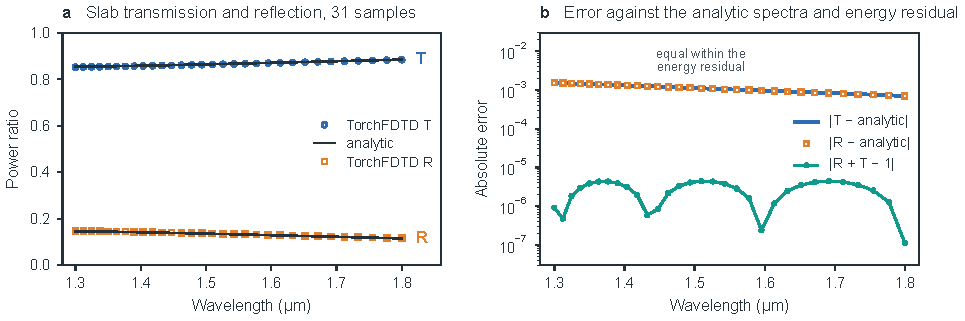
\includegraphics[width=\linewidth]{figures/flux-validation.pdf}
\caption{Plane-monitor spectra of the lossless slab against Eq.~\eqref{eq:slab}. Absolute errors of the 31 recorded samples are plotted on the logarithmic right axis.}
\label{fig:flux-validation}
\end{figure}

A closed total-field/scattered-field box around a dielectric sphere yields the scattering cross-section over nine wavelengths, which is compared with the Mie series \citep{bohren1983}. The error over a mesh sequence is not monotonic: it falls from 8.9\% at a 0.1~\micron{} mesh to 0.31\% at 0.05~\micron{}, rises to 1.05\% at 0.025~\micron{} and falls again to 0.55\% at 0.02~\micron{}, while doubling the physical duration leaves the 0.025~\micron{} value unchanged (Table~\ref{tab:tfsf-sphere}, Fig.~\ref{fig:tfsf-sphere}). The staircased sphere surface, not the box or the duration, sets this error.

% Generated by scripts/build_paper_assets.py from native validation JSON.
\begin{table}[tbp]
\centering
\small
\renewcommand{\arraystretch}{1.15}
\caption{Closed-box TFSF sphere scattering on RTX 5880. The maximum relative cross-section error is taken over nine wavelengths. Physical domain and PML thickness stay fixed. The final row doubles the physical duration. The error sequence is not monotonic.}
\label{tab:tfsf-sphere}
\begin{tabular}{@{}lrrrr@{}}
\toprule
$h$ ($\mu$m) & Grid & \shortstack{Time\\(fs)} & \shortstack{Max error\\(\%)} & \shortstack{Empty box\\($\mu$m$^2$)} \\
\midrule
0.1 & $32^3$ & 120 & 8.8963 & $6.68\times10^{-15}$ \\
0.05 & $64^3$ & 120 & 0.3086 & $1.11\times10^{-14}$ \\
0.025 & $128^3$ & 120 & 1.0474 & $2.19\times10^{-15}$ \\
0.02 & $160^3$ & 120 & 0.5514 & $1.37\times10^{-14}$ \\
0.025 & $128^3$ & 240 & 1.0474 & $2.32\times10^{-15}$ \\
\bottomrule
\end{tabular}
\end{table}


\begin{figure}[tbp]
\centering
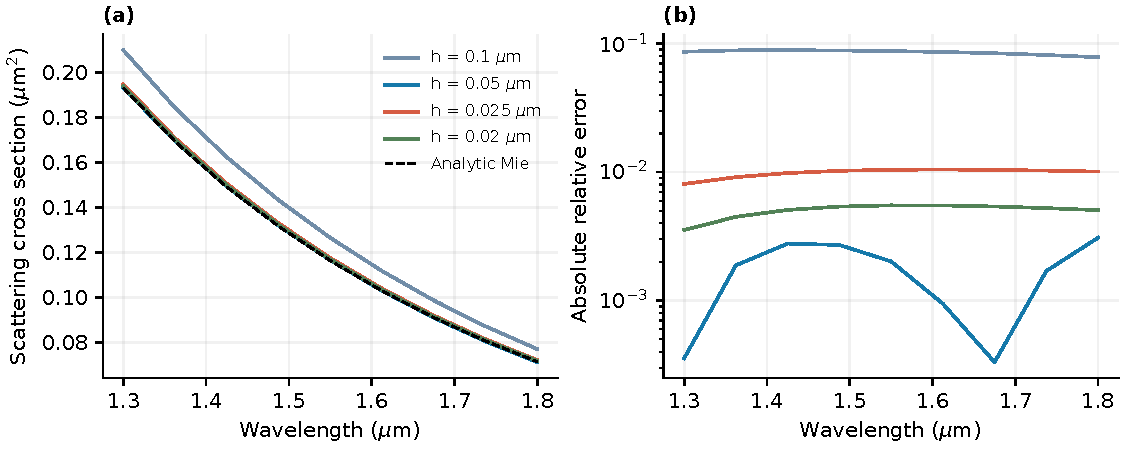
\includegraphics[width=\linewidth]{figures/tfsf-sphere.pdf}
\caption{Scattering cross-section of the dielectric sphere from the closed total-field/scattered-field box at four mesh steps, with the Mie series as reference.}
\label{fig:tfsf-sphere}
\end{figure}

Radiation projections are checked against the closed-form fields of an electric dipole. With 14, 28 and 56 samples per face axis the finite-distance projection reaches relative errors of $4.6\times10^{-3}$, $1.1\times10^{-3}$ and $2.8\times10^{-4}$ at five points between 0.55 and 1.35~\micron{} outside the box, a second-order sequence, and the asymptotic and finite-distance models agree to $1.9\times10^{-4}$ at a radius of 2000~\micron{}. A lossy exterior with index $1.3+0.05\mathrm{i}$ reproduces the analytic near and far fields with the same convergence. For an open surface the single-face projection of a Gaussian-apodized directional emitter converges to the closed-box result as the field on the omitted faces decays, from $9.6\times10^{-2}$ to $3.8\times10^{-3}$ as the beam waist grows from 0.4 to 0.8 wavelengths, whereas an isotropic dipole stays at 0.79 under refinement.

Guided-mode ports are validated on a straight guide, an interface between guides of index 1.0 and 1.2 whose complex scattering parameters are compared with an independent discrete interface solution, a symmetric Y branch and a four-port crossing. A narrow-aperture port on a wide domain matches the full-cell network to $1.6\times10^{-5}$ in the scattering parameters, the Y branch obeys reciprocity to $2.0\times10^{-3}$ with a $1.2\times10^{-4}$ arm asymmetry, and the crossing obeys reciprocity to $2.4\times10^{-4}$ with a $1.2\times10^{-7}$ gap between its four-fold rotated columns. The power missing from the guided channels of the Y branch is radiated by the staircased junction and is reported as a defect rather than corrected.

The anisotropic path is checked against a birefringent slab of principal indices 1.5 and 2.0 in a co-aligned exterior of indices 1.2 and 1.4 that fills both absorbing faces along the propagation axis. The two polarization channels reproduce the analytic transmission to 1.37\% and 0.33\%, and the derivative of the transmission with respect to the slab index agrees with the analytic derivative to 6.9\%. A magnetic wall next to an absorbing face reflects $1.7\times10^{-4}$ of the incident power with the default profile and $3.5\times10^{-4}$ with $\kappa=3$, $\alpha=0.05$ and a quadratic grading.

\subsection{Gradient checks}

Every differentiable path is compared with full Torch automatic differentiation on a small grid and with central differences along a random direction, and the Taylor remainder of the directional derivative is required to fall quadratically. Table~\ref{tab:gradients} lists the recorded agreement. The material gradient of the $256^{3}$ problem of Section~\ref{sec:performance} agrees with the complete-history reference to a relative $L_2$ error of $2.4\times10^{-7}$ for the dielectric and $4.3\times10^{-7}$ for the two-pole material, both in single precision.

\begin{table}[tbp]
\centering
\small
\renewcommand{\arraystretch}{1.15}
\caption{Recorded gradient agreement of the discrete adjoint. Relative errors compare the transposed sweep with full Torch automatic differentiation unless a finite-difference (FD) reference is named. FP64 on CPU unless stated.}
\label{tab:gradients}
\begin{tabular}{@{}llr@{}}
\toprule
Path & Reference & Relative error \\
\midrule
Polygon solid through the checkpointed adjoint & autograd, CUDA FP32 & $1.2\times10^{-7}$ \\
Magnetic-wall faces with CPML & autograd & $2\times10^{-16}$ \\
Dispersive faces, four pole parameters & autograd & $2.7\times10^{-16}$ \\
Polygon vertices, voxel VJP & central FD, CPU and CUDA & $6.7\times10^{-8}$ \\
Polygon vertices through the solver & central FD & $4.4\times10^{-9}$ to $5.5\times10^{-8}$ \\
Spline control points & central FD & $1.8\times10^{-8}$ \\
Modal $|S_{21}|^{2}$ objective, N-port & autograd, CPU and CUDA & $1.3\times10^{-15}$ to $5.4\times10^{-15}$ \\
Far-field intensity objective & central FD & $3.4\times10^{-10}$ \\
Near-zone Poynting objective & central FD & $2.7\times10^{-9}$ \\
Streamed versus resident, tensor media & resident sweep & $1\times10^{-10}$ \\
Streamed versus resident, magnetic walls & resident sweep & $3\times10^{-7}$ \\
\bottomrule
\end{tabular}
\end{table}

The discrete adjoint of a shape parameter converges to the physical shape derivative only with the mesh. For a two-dimensional pentagon grating of permittivity 4 and period 0.6~\micron{} at normal incidence and 1.55~\micron{}, the vertex gradient at mesh steps of 0.04, 0.02 and 0.01~\micron{} differs from a central-difference reference at 0.005~\micron{} by 11.6\%, 1.8\% and 0.5\% for a 0.08~\micron{} smoothing width, and by 5.4\% and 1.0\% at the two coarser steps for a 0.04~\micron{} width. Halving the reference step moves the reference by less than 0.07\%.

\subsection{Test suite}

The behaviour above is fixed by 2,141 tests that run on a Linux CPU continuous-integration host and on two CUDA workstations, and every device path is compared with its CPU counterpart. Recorded numerical fixtures carry the SHA-256 of the source files that produced them, so a change in a kernel that alters a recorded number is caught by the test that reads the record.

\section{Performance}
\label{sec:performance}

All timings below were taken on one NVIDIA RTX 5880 Ada with 48 GiB (51.5 GB) of device memory in a Windows workstation with 137 GB of host memory, in single precision unless stated, as medians of three warmed repetitions that include construction, graph capture, stepping and the transfer of the final fields. Cold compilation and disk writes are excluded.

\subsection{Single simulations and ensembles}

The fused engine is compared with the PyTorch FDTD package it builds on, executed through the same CUDA Graph adapter so that both run without Python in the step loop \citep{fdtd}. Over eight fixtures at $64^{3}$ and $96^{3}$ cells and 800 steps the fused kernels are 15.8 to 17.1 times faster at $64^{3}$ and 9.6 to 12.1 times faster at $96^{3}$, with point-trace differences below 0.04\% that arise from the different absorber stencils (Table~\ref{tab:open-source}). Sixteen-case parameter sweeps run 31 to 44 times faster than the sequential upstream package at $32^{3}$ and 15 to 16 times faster at $64^{3}$ when the cases share one tensor batch, and four sphere cases at $64^{3}$ and 800 steps take 1.18 s with one CUDA worker against 47.0 s with one NumPy worker (Fig.~\ref{fig:batch-throughput}). The tensor batch itself is 2.4 times faster than sequential native execution for sixteen $32^{3}$ cases and slower than sequential execution for sixteen $64^{3}$ cases, so cohorts of four are selected at that size (Table~\ref{tab:tensor-batch}).

% Generated by scripts/build_paper_assets.py from native validation JSON.
\begin{table}[tbp]
\centering
\small
\renewcommand{\arraystretch}{1.15}
\caption{Eight forward fixtures on RTX 5880. The external baseline is flaport/fdtd 0.2.2 with an added CUDA Graph adapter. Values are medians of three warmed full solves. The last column is point-trace relative L2 difference in percent, not analytic error. The PML interface stencils differ and final fields are not identical.}
\label{tab:open-source}
\begin{tabular}{@{}lrrrr@{}}
\toprule
Fixture, grid & \shortstack{Upstream graph\\(ms)} & \shortstack{Native fused\\(ms)} & Speedup & \shortstack{Trace L2\\(\%)} \\
\midrule
Vacuum, $64^3$ & 649.23 & 38.06 & $17.06\times$ & 0.0142 \\
Sphere, $64^3$ & 629.07 & 39.72 & $15.84\times$ & 0.0233 \\
Slab, $64^3$ & 636.26 & 37.23 & $17.09\times$ & 0.0197 \\
Waveguide, $64^3$ & 632.59 & 39.90 & $15.85\times$ & 0.0372 \\
Vacuum, $96^3$ & 954.98 & 78.77 & $12.12\times$ & 0.0120 \\
Sphere, $96^3$ & 848.58 & 88.05 & $9.64\times$ & 0.0208 \\
Slab, $96^3$ & 836.66 & 80.37 & $10.41\times$ & 0.0174 \\
Waveguide, $96^3$ & 848.07 & 80.00 & $10.60\times$ & 0.0328 \\
\bottomrule
\end{tabular}
\end{table}

% Generated by scripts/build_paper_assets.py from native validation JSON.
\begin{table}[tbp]
\centering
\small
\renewcommand{\arraystretch}{1.15}
\caption{Native sphere ensembles on RTX 5880 with a real CUDA batch axis. Full wall times include setup, transfers and scalar objective evaluation. Final E/H arrays and point traces match independent native runs bitwise. Values below unity in the last column are slowdowns.}
\label{tab:tensor-batch}
\begin{tabular}{@{}lrrrr@{}}
\toprule
Grid, cases & \shortstack{Sequential\\(ms)} & \shortstack{Tensor cohort\\(ms)} & Cases/s & Speedup \\
\midrule
$32^3$, 1 & 23.22 & 20.38 & 49.06 & $1.14\times$ \\
$32^3$, 2 & 46.00 & 31.39 & 63.71 & $1.47\times$ \\
$32^3$, 4 & 106.81 & 63.67 & 62.83 & $1.68\times$ \\
$32^3$, 8 & 181.89 & 88.24 & 90.66 & $2.06\times$ \\
$32^3$, 16 & 341.29 & 142.46 & 112.31 & $2.40\times$ \\
$64^3$, 1 & 39.08 & 40.49 & 24.70 & $0.97\times$ \\
$64^3$, 2 & 86.40 & 78.29 & 25.55 & $1.10\times$ \\
$64^3$, 4 & 167.68 & 153.87 & 26.00 & $1.09\times$ \\
$64^3$, 8 & 307.35 & 357.10 & 22.40 & $0.86\times$ \\
$64^3$, 16 & 669.53 & 852.94 & 18.76 & $0.78\times$ \\
\bottomrule
\end{tabular}
\end{table}


\begin{figure}[tbp]
\centering
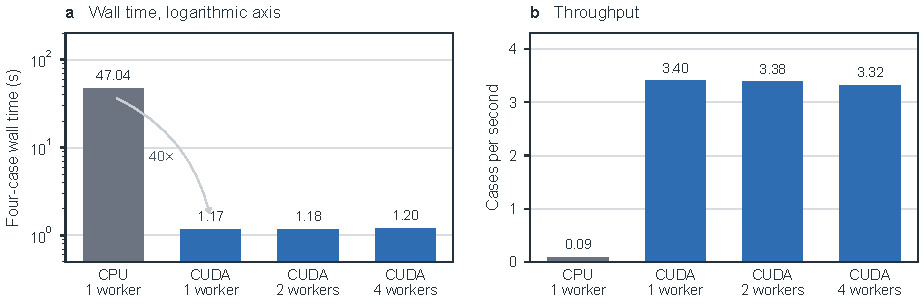
\includegraphics[width=\linewidth]{figures/batch-throughput.pdf}
\caption{Wall time and throughput of four-structure ensembles. Bars are medians of three measured batches after warm-up and the left axis is logarithmic.}
\label{fig:batch-throughput}
\end{figure}

\subsection{Adjoint}

A $256^{3}$ problem with 128 steps and two checkpoints, timed from construction through the plane-flux objective and every material cotangent, takes 407.7 s for a dielectric and 742.0 s for a two-pole material on the same Torch model with twelve CPU threads, 2.28 s and 5.00 s resident on the device, and 9.44 s and 23.9 s in the streamed mode with host banks. The resident device adjoint is therefore 179 and 149 times faster than the CPU model, and the streamed mode retains 43 and 31 of those factors while holding only the active slabs on the device.

\subsection{Beyond the device memory}

Two runs exceed the 51.5 GB of the processor. The first advances a $1152\times1024\times2048$ real single-precision grid of 2.42 billion cells, whose electric and magnetic state occupies 58.0 GB and 58.3 GB with the absorber memories, for ten steps and a full spatial permittivity gradient with file banks on solid-state storage. The peak device allocation is 2.23 GB, the process peak resident memory is 31.9 GB, the run completes in 58.4 minutes, and the gradient over the causal cone of a point source agrees with a reference computed on the cone alone to a relative $L_2$ error of $9.1\times10^{-8}$ while no cell outside the cone receives a gradient.

The second run tests the journal on a $1152\times1024\times1920$ grid of 2.26 billion cells with the same policy and one journal record per block (Table~\ref{tab:restart}). The first process exits deliberately after publishing its first backward record. A second process restores the completed forward signals in 7.7 s, resumes the backward sweep below the recorded block and finishes in 957 s with a peak device allocation of 3.03 GB, and its gradient matches the causal-cone reference to $9.08\times10^{-8}$. Whole-machine counters sampled every five seconds over both processes peak at 38.9 GB in use of 137 GB installed, with a mean disk write rate of 0.59 GB/s and 1.52 TB written in total, so the operating-system file cache stays below 0.3 GB because every bank is written and read once per block.

\begin{table}[tbp]
\centering
\small
\renewcommand{\arraystretch}{1.15}
\caption{Interrupted and resumed single-precision adjoint on the $1152\times1024\times1920$ grid with slab width 4, temporal depth 4, no interior checkpoints, file banks and one journal record per block.}
\label{tab:restart}
\begin{tabular}{@{}lrr@{}}
\toprule
 & Killed process & Resumed process \\
\midrule
Forward sweep (s) & 559.1 & 7.7 (restored) \\
Journal writes (s) & 96.6 & 64.8 \\
Total elapsed (s) & 1137.4 & 957.5 \\
Peak device allocation (GB) & & 3.03 \\
Peak process resident memory (GB) & 28.5 & 30.0 \\
Backward file traffic, read / written (GB) & & 546 / 437 \\
Gradient relative $L_2$ error & & $9.08\times10^{-8}$ \\
\bottomrule
\end{tabular}
\end{table}

\section{Discussion}

We demonstrate a time-domain solver in which the same fused CUDA kernels serve the forward run, its transposed sweep and a streamed execution whose field state exceeds the memory of the processor, with a device footprint of 2 to 3 GB for a 54 GB problem. The measured reservations and the journal turn a large adjoint from a single fragile allocation into a sequence of block records that can be planned, budgeted and resumed.

The design of the differentiation layer separates it from frameworks that differentiate their own operations. TORCWA and FDTDX obtain gradients from the framework at the cost of keeping every differentiated operation inside it \citep{kim2023,mahlau2024}, whereas TorchFDTD pays that cost once, in the transposes of a small set of kernels, and is then free to fuse, tile and offload. The price is coverage: a new physical update needs its transpose before it becomes differentiable, and the eigenmode solver and the source positions are held fixed here as they are in the frameworks above. Single-domain multi-GPU execution is implemented on CPU ranks and awaits a validation on two devices.

Several directions follow from the records. The tensor and magnetic-wall paths run their transposes as Torch operations rather than as fused kernels, so their device throughput is bounded by memory traffic that the fused isotropic kernels avoid. The staircase junction of the Y branch and the non-monotonic sphere errors point to the subpixel operator as the next accuracy step for curved and angled interfaces. Sustained throughput of the streamed mode over hours, rather than the ten-step capacity gates recorded here, will decide how far a single workstation can carry an inverse design whose state exceeds its device.

\section{Conclusion}

TorchFDTD provides an FDTD engine whose forward kernels, transposes and storage tiers are designed together, so that inverse design on one graphics processor is limited by host memory and storage rather than by device memory. The package, its validation records and the source hashes of every measurement are available under the MIT licence \citep{torchfdtd}. Extending the fused transposes to tensor media and magnetic walls, measuring multi-device execution on real hardware, and running the streamed adjoint through a complete multi-hour optimization are the next steps toward design problems of ten billion cells on a single workstation.

\section*{Data and code availability}

The source code, the browser workbench, the test suite and every JSON record quoted in this paper are in the public repository \citep{torchfdtd}. Each record stores the SHA-256 of the source files that produced it and the hardware on which it was taken.

\bibliographystyle{unsrtnat}
\bibliography{references}

\end{document}
